\documentclass[main.tex]{subfiles}
\usepackage{listings}
\begin{document}
\begin{enumerate}

\subsection*{Section 7}
	
\item[19.] Answer the following questions about LANs (wired and wireless):

    \begin{enumerate}
        \item \textbf{Q.} Describe (through some pseudo code and sufficient explanation) CSMA/CD and Binary Exponential Backoff as used in IEEE 802.3 Ethernet. \textbf{A.} CSMA/CD stands for Carrier Sense Multiple Access with Collision Detection, which is a protocol used in IEEE 802.3 Ethernet to regulate data transmission on a shared medium. The basic idea of CSMA/CD is that each station (sender) first senses the medium (cable) before sending a data frame. If the medium is busy, the station waits until it becomes idle. If the medium is idle, the station starts sending the frame and monitors the medium for any collision (interference) with other frames. If a collision is detected, the station stops sending the frame and waits for a random amount of time before trying again. This random time is determined by a binary exponential backoff algorithm, which increases the range of possible waiting times after each collision. The pseudo code for CSMA/CD and binary exponential backoff can be written as follows:

\begin{verbatim}
# Define some constants
MAX_ATTEMPTS = 16 # Maximum number of attempts before giving up
SLOT_TIME = 51.2 microseconds # one bit propagate the max cable length
MIN_BACKOFF = 0 # Minimum backoff factor
MAX_BACKOFF = 10 # Maximum backoff factor

# Define a function to sense the medium
function sense_medium():
  return True if medium is idle, False if medium is busy

# Define a function to send a frame
function send_frame(frame):
  # Initialize some variables
  attempt = 0 # Number of attempts so far
  success = False # Whether the frame has been sent successfully
  collision = False # Whether a collision has been detected

  # Repeat until success or maximum attempts reached
  while not success and attempt < MAX_ATTEMPTS:
    # Sense the medium
    if sense_medium():
      # Start sending the frame and monitor the medium
      start_sending(frame)
      while not done_sending(frame):
        if sense_medium():
          # No collision, continue sending
          continue
        else:
          # Collision detected, stop sending and set collision flag
          stop_sending(frame)
          collision = True
          break
      
      # Check if collision occurred
      if collision:
        # Increment the attempt counter and calculate the backoff factor
        attempt = attempt + 1
        backoff = random_integer(MIN_BACKOFF, min(MAX_BACKOFF, attempt))
        
        # Wait for a random number of slot times 
        # based on the backoff factor
        wait_time = backoff * SLOT_TIME
        wait(wait_time)
        
        # Reset the collision flag and try again
        collision = False
      else:
        # No collision, frame sent successfully and set success flag
        success = True
    
    else:
      # Medium is busy, wait for one slot time and try again
      wait(SLOT_TIME)
  
  # Return success or failure status
  return success
\end{verbatim}

        The binary exponential backoff algorithm works by choosing a random integer between 0 and $2^{\wedge} \mathrm{i}-1$, where $\mathrm{i}$ is the number of attempts so far, bounded by a maximum value. This integer is multiplied by the slot time, which is the time it takes for one bit to propagate across the maximum cable length. The resulting time is the waiting time before trying to send again. The algorithm ensures that after each collision, the probability of another collision decreases, as the stations are more likely to choose different waiting times. However, if the number of attempts exceeds a maximum value (usually 16), the station gives up and reports a failure.

        \item \textbf{Q.} Describe CSMA/CA (through some pseudo code and sufficient explanation) as used in IEEE 802.11 WiFi. \textbf{A.} Carrier Sense Multiple Access with Collision Avoidance (CSMA/CA) is a network multiple access method in which carrier sensing is used, but nodes attempt to avoid collisions by beginning transmission only after the channel is sensed to be "idle". CSMA/CA is a protocol that operates in the data link layer (Layer 2) of the OSI model 1.In IEEE 802.11 WiFi, CSMA/CA is used to improve the performance of the CSMA method by attempting to divide the channel somewhat equally among all transmitting nodes within the collision domain. The simplified algorithm of CSMA/CA is as follows :
        \begin{enumerate}
            \item Carrier Sense: prior to transmitting, a node first listens to the shared medium (such as listening for wireless signals in a wireless network) to determine whether another node is transmitting or not. Note that the hidden node problem means another node may be transmitting which goes undetected at this stage.
            \item Collision Avoidance: if another node was heard, we wait for a period of time (usually random) for the node to stop transmitting before listening again for a free communications channel. Request to Send/Clear to Send (RTS/CTS) may optionally be used at this point to mediate access to the shared medium. This goes some way to alleviating the problem of hidden nodes because, for instance, in a wireless network, the Access Point only issues a Clear to Send to one node at a time. However, wireless 802.11 implementations do not typically implement RTS/CTS for all transmissions; they may turn it off completely, or at least not use it for small packets (the overhead of RTS, CTS and transmission is too great for small data transfers).
            \item Transmission: if the medium was identified as being clear or the node received a CTS to explicitly indicate it can send, it sends the frame in its entirety. Unlike CSMA/CD, it is very challenging for a wireless node to listen at the same time as it transmits (its transmission will dwarf any attempt to listen). Continuing the wireless example, the node awaits receipt of an acknowledgement packet from the Access Point to indicate the packet was received and checksummed correctly. If such acknowledgement does not arrive in a timely manner, it assumes the packet collided with some other transmission, causing the node to enter a period of binary exponential backoff prior to attempting to re-transmit.
        \end{enumerate}

\begin{verbatim}
    # CSMA/CA simplified pseudo-code 
    N=1 
    while N<= max : 
        waitUntil(free(channel)) 
        if correct(last_frame) : 
          wait(channel_free_during_t >=DIFS) 
        else: 
          wait(channel_free_during_t >=EIFS) 
    
        back-off_time = int(random[0,min(255,7*(2^(N-1)))])*slotTime 
        wait(channel free during backoff_time) 
        # backoff timer is frozen while channel is sensed to be busy 
        send(frame) 
        wait(ack or timeout) 
        if received(ack) 
          # frame received correctly 
          break 
        else: 
          # retransmission required 
          N=N+1 
\end{verbatim}
        
    \end{enumerate}
    
\item[20.] \textbf{Q.} M terminals are attached by a dedicated pair of lines to a hub in a star topology (Figure \ref{fig:20q_a}). The distance from each terminal to the hub is d meters, the speed of the transmission lines is R bits/second, all frames are f length 12,500 Bytes, and the signal propagates on the line at speed of $2.5^{*} 10^{8}$ meters/second. For M=6 terminals, d=25 meters and R = 10Gbps, what is the maximum network throughput achievable when the hub is implementing slotted ALOHA? 

\begin{figure}
\centering\fbox{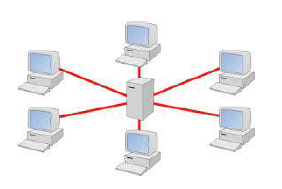
\includegraphics[width=3.0in]{2018spring/figures/20q_a.png}}
\caption{Star Topology}
\label{fig:20q_a}
\end{figure}

\textbf{Theory.} Slotted ALOHA is an improved version of the pure ALOHA protocol that aims to make communication networks more efficient. In this version, the channel is divided into small, fixed-length time slots and users are only allowed to transmit data at the beginning of each time slot. This synchronization of transmissions reduces the chances of collisions between devices, increasing the overall efficiency of the network. To calculate the throughput of Slotted ALOHA let $\mathrm{T}$ be the frame time, i.e. the time required for 1 frame to be transmitted. Let $\mathrm{G}$ be the number of transmission attempts per frame time. The probability that $k$ frames are generated during the frame time is given by the Poisson distribution-

$$
P(k)=\frac{G^k e^{-G}}{k !}
$$

From this we can say that the probability that 0 frames are generated $(k=0)$ during the frame time is $e^{-G}$. In case of slotted ALOHA, the vulnerable time period for collision between two frames is equal to time duration of 1 slot, which is equal to 1 frame time, i.e. $T$. In $T$ time, average number of transmission attempts is $\mathrm{G}$. The probability that 0 frames are initiated in the vulnerable time period will be

$$
P(0)=e^{-G}
$$

The throughput, $S$, is calculated as the number of transmission attempts per frame time, $G$, multiplied by the probability of success, $P P(0)$.

$$
S=G \cdot P(0)
$$

or

$$
S=G e^{-G}
$$

The maximum throughput of Slotted ALOHA occurs when $\mathrm{G}=1$. The maximum throughput is thus

$$
S_{\max }=1 \times e^{-1}=\frac{1}{e}=0.368
$$

Thus, it can be seen that the maximum throughput is $36.8 \%$ in slotted ALOHA,which is an improvement over maximum throughput of $18.4 \%$ in pure ALOHA. Throughput $(s)=G \times e-G$. The maximum Throughput occurs at $G=1$, i.e. $S=1 / e=0.368$. Where: $\mathrm{G}=$ the offered load (or the number of packets being transmitted per time slot). The offered load is a measure of the number of nodes attempting to transmit in a given time slot. The throughput is a function of the offered load and it ranges from 0 to 1. As the offered load increases, the throughput decreases as more collisions occur, resulting in less successful transmissions. The maximum throughput is achieved when the offered load is equal to 0.37 and it is approximately 0.184. It is important to note that the above equation assumes that all the packets are of the same length and that the channel is error-free. In practice, the throughput is usually much lower than this due to a number of factors such as packet errors, channel noise, and the overhead of re transmissions.

\textbf{A.} The maximum network throughput achievable can be calculated as,

$$
\rho_{\max }=\frac{1}{e} \times\left[\frac{R \mathrm{bits} / \mathrm{s}}{L \text { bits } / \text { packet }}\right]=z \text { packets } / \text { sec }
$$

For $M=6$ terminals, $d=25$ meters and $R=10 \mathrm{Gbps}$, we can calculate the offered load as follows. The time taken for a signal to travel from a terminal to the hub is 

$$
\frac{\mathrm{d}}{(2.5\times 10^{8} \si{m.s^{-1}})}
$$ 

seconds. The time taken for a frame of length $f=12500$ Bytes to be transmitted is 

$$
\frac{12500 \times 8}{R}
$$ 

seconds. The number of frames that can be transmitted per second is 

$$
\frac{\mathrm{R}}{(12500 \times 8)}
$$

frames/second. Therefore, the number of frames that can be transmitted in 

$$
\frac{\mathrm{d}}{(2.5\times 10^{8} \si{m.s^{-1}})}
$$ 

seconds is 

$$
\frac{\mathrm{R}}{(12500 \times 8)} * \frac{\mathrm{d}}{(2.5\times 10^{8} \si{m.s^{-1}})}
$$ 

frames. The offered load is the number of frames being transmitted per time slot which is equal to 

$$
\frac{1}{M}\left(\frac{\mathrm{R}}{(12500 \times 8)} * \frac{\mathrm{d}}{(2.5\times 10^{8} \si{m.s^{-1}})}\right)
$$ 

frames/time slot. Substituting M=6, $d=25$ meters and $R=10 \mathrm{Gbps}$ in the above formula gives us an offered load of approximately $\mathbf{0.0000000004}$ frames/time slot. Substituting this value in the formula for maximum throughput gives us a maximum throughput of approximately $0.00000000015$ or $1.5 \times 10^{-10}$.


\item[21.] Consider a data link layer with the following parameters: Frame transmission time at the sender is $\mathrm{t}_\mathrm{f}=20$ microseconds. ACK or NAK transmission time at the receiver is $\mathrm{t}_\mathrm{ack} = 10$ microseconds. Link propagation delay on both directions is $\mathrm{t}_{\mathrm{prop}} = 25$ microseconds. Suppose frame processing time at both sender and receiver is negligible, i.e., $\mathrm{t}_{\mathrm{prop}] = 0$. Finally, overall round-trip probability of frame error on the link is $r=0.04$. 

    \begin{enumerate}
        \item Assume that for the Stop-and-wait ARQ scheme, the TIMEOUT at the sender is chosen optimally. What is the resulting throughput (frames/second)?
        \item  In the Go-Back-N ARQ scheme, if the link is error free, what is the minimum window size $N$ that is able to keep the link busy?
        \item Choose window size in Part b and now consider the link error probability $r=0.04$. What the throughput (frames/second) of the Go-Back-N ARQ scheme?
    \end{enumerate}

\end{enumerate}
\end{document}